\documentclass[11pt]{article}
\usepackage[margin=1in]{geometry}
\usepackage{amsmath,amssymb,amsthm}
\usepackage{booktabs}
\usepackage{graphicx}
\usepackage{hyperref}
\usepackage{enumitem}
\graphicspath{{../docs/figures/}}
\newcommand{\ExpOneSeeds}{20}
\newcommand{\ExpOneWins}{20/20}
\newcommand{\ExpOneBestBaseline}{SGD + momentum, cosine lr}
\newcommand{\ExpOneBaselineGap}{9.7\times 10^{-8}}
\newcommand{\ExpOneSvrgGap}{4.1\times 10^{-31}}
\newcommand{\ExpOneBaselineRange}{$8.3\times 10^{-8}$ to $2.8\times 10^{-7}$}
\newcommand{\ExpFourWins}{12/12}
\newcommand{\ExpSixAdaptiveVsMomentum}{{-}1.5}
\newcommand{\ExpSixAdaptiveCI}{[{-}2.0, {-}1.1]}
\newcommand{\ExpSixAdaptiveWins}{20/20}
\newcommand{\ExpSixCosineVsAdamCosine}{{-}5.3}
\newcommand{\ExpSixCosineCI}{[{-}6.6, {-}4.9]}
\newcommand{\ExpSixCosineWins}{20/20}
\newcommand{\ExpSixConstGap}{6.8\times 10^{-4}}
\newcommand{\ExpSixCosineGap}{3.5\times 10^{-11}}
\newcommand{\ExpSixAdamCosineGap}{5.9\times 10^{-6}}
\newcommand{\ExpFiveN}{40000}
\newcommand{\ExpFiveD}{200}
\newcommand{\ExpFiveSvrgSeconds}{0.08}
\newcommand{\ExpFiveNormalSeconds}{0.06}
\newcommand{\ExpFiveLstsqSeconds}{0.48}
\newcommand{\ExpSevenDecades}{{-}1.3}
\newcommand{\ExpSevenWins}{8/8}
\newcommand{\ExpEightGap}{+0.0135}
\newcommand{\ExpEightCI}{[+0.0106, +0.0150]}
\newcommand{\ExpEightSvrgTest}{0.1445}
\newcommand{\ExpEightBaselineTest}{0.1317}
\newcommand{\ExpEightSvrgTrain}{0.1079}
\newcommand{\ExpEightBaselineTrain}{0.1177}
\newcommand{\ExpEightBaselineName}{SGD + momentum, cosine lr}
\newcommand{\ExpEightLogisticLow}{0.68775}
\newcommand{\ExpEightLogisticHigh}{0.68776}
\newcommand{\ExpEightAccuracy}{54}
\newcommand{\ExpTwoVrStart}{2.6\times 10^{-1}}
\newcommand{\ExpTwoVrEnd}{9.9\times 10^{-16}}
\newcommand{\ExpTwoSgdMin}{1.7}
\newcommand{\ExpTwoSgdMax}{2.5}
\newcommand{\ExpTwoProbes}{25}
\newcommand{\ExpTwoWithinLemma}{100}
\newcommand{\ExpTwoWithinProp}{100}
\newcommand{\ExpNineBestK}{64}
\newcommand{\ExpNineBestEvals}{60{,}800}
\newcommand{\ExpNineMaxRatio}{2.2\times 10^{-4}}
\newcommand{\ExpNineKmin}{8}
\newcommand{\ExpNineKmax}{1024}
\newcommand{\ExpNineWithinTwoLow}{16}
\newcommand{\ExpNineWithinTwoHigh}{64}
\newcommand{\ExpNineMidFactor}{2.1}
\newcommand{\ExpNineSmallFactor}{2.2}
\newcommand{\ExpNineLargeFactor}{5.6}
\newcommand{\ExpTenBadRaw}{1.1\times 10^{7}}
\newcommand{\ExpTenBadJacobi}{82}
\newcommand{\ExpTenGoodRaw}{81}
\newcommand{\ExpTenGoodJacobi}{82}
\newcommand{\ExpElevenBadTheoryGap}{2.6\times 10^{-29}}
\newcommand{\ExpElevenBadTunedGap}{1.8\times 10^{-29}}
\newcommand{\ExpElevenGoodTheoryGap}{6.2\times 10^{-30}}
\newcommand{\ExpElevenAlpha}{0.50}
\newcommand{\ExpElevenContractionBad}{0.08}
\newcommand{\ExpElevenContractionGood}{0.10}
\newcommand{\ExpElevenInner}{4{,}139}
\newcommand{\ExpElevenEvalsTheory}{73{,}848}
\newcommand{\ExpElevenEvalsTuned}{49{,}152}
\newcommand{\ExpElevenEvalsCoord}{348{,}288}
\newcommand{\ExpElevenSpeedup}{4.7}
\newcommand{\ExpElevenBadWins}{20/20}
\newcommand{\ExpTwelveJacobiGap}{9.7\times 10^{-30}}
\newcommand{\ExpTwelveCoordGap}{7.4\times 10^{-19}}
\newcommand{\ExpTwelveWins}{12/12}
\newcommand{\ExpTwelveEvalsJacobi}{169{,}152}
\newcommand{\ExpTwelveEvalsCoord}{485{,}296}
\newcommand{\ExpTwelveSpeedup}{2.9}
\newcommand{\ExpTwelveAdamCosineGap}{8.7\times 10^{-7}}
\newcommand{\ExpTwelveAdaptiveVsMomentum}{{-}9.3}
\newcommand{\ExpTwelveSeeds}{12}
\newcommand{\ExpThirteenMinDiff}{0.06}
\newcommand{\ExpThirteenMaxDiff}{0.52}
\newcommand{\ExpThirteenBCDecades}{5.3}
\newcommand{\ExpThirteenBCCondRaw}{3.1\times 10^{7}}
\newcommand{\ExpThirteenBCCondJacobi}{2.5\times 10^{5}}
\newcommand{\ExpThirteenBCGap}{6.0\times 10^{-3}}
\newcommand{\ExpThirteenWineGap}{1.7\times 10^{-3}}
\newcommand{\ExpThirteenWineBaseline}{5.7\times 10^{-3}}
\newcommand{\ExpThirteenAnyReached}{no}
\newcommand{\ExpFourteenAligned}{5.1\times 10^{-5}}
\newcommand{\ExpFourteenMisaligned}{3.4}
\newcommand{\ExpFourteenSgd}{1.6}
\newcommand{\ExpFourteenRatio}{2.1}
\newcommand{\ExpFourteenNaiveFinite}{76}
\newcommand{\ExpFourteenClampFinite}{76}
\newcommand{\ExpFourteenFullFinite}{0}
\newcommand{\ExpFourteenNaiveInf}{100}
\newcommand{\ExpFourteenTrials}{2{,}000}
\newcommand{\ExpFifteenAdaptiveDiff}{+0.0038}
\newcommand{\ExpFifteenAdaptiveCI}{[+0.0032, +0.0044]}
\newcommand{\ExpFifteenMomentumDiff}{+0.0000}
\newcommand{\ExpFifteenMomentumCI}{[{-}0.0001, +0.0007]}
\newcommand{\ExpFifteenAdamVsSgd}{+0.0012}
\newcommand{\ExpFifteenBaselineName}{SGD + momentum, cosine lr}
\newcommand{\ExpSixteenSvrgReached}{3/3}
\newcommand{\ExpSixteenBaselineReached}{0/3}
\newcommand{\ExpSixteenBaselineLow}{6.1\times 10^{-8}}
\newcommand{\ExpSixteenBaselineHigh}{1.8\times 10^{-2}}
\newcommand{\ExpSixteenSvrgHigh}{2.2\times 10^{-20}}
\newcommand{\ExpSixteenCondBC}{140}
\newcommand{\ExpSixteenCondWine}{34}
\newcommand{\ExpSixteenCondDiabetes}{470}
\newcommand{\LatDot}{15\,ns}
\newcommand{\LatRls}{959\,ns}
\newcommand{\LatSvrgOne}{129\,ns}
\newcommand{\LatSvrgBatch}{3.9\,$\mu$s}
\newcommand{\LatSnapshot}{1.8\,ms}
\newcommand{\LatWindow}{100{,}000}
\newcommand{\LatRlsOverSvrgHundredTwentyEight}{43}
\newcommand{\LatDiffErr}{3.3\times 10^{-16}}
\newcommand{\LatCpu}{Intel Xeon @ 2.10GHz}
\newcommand{\ExpThreeMaxICDiff}{0.0054}
\newcommand{\ExpThreeIQR}{0.08}


\newtheorem{lemma}{Lemma}
\newtheorem{proposition}{Proposition}
\theoremstyle{remark}
\newtheorem*{remark}{Remark}

\newcommand{\E}{\mathbb{E}}
\newcommand{\norm}[1]{\lVert #1\rVert}
\newcommand{\ghat}{\hat g}

\title{Coordinate-wise SVRG for Low Signal-to-Noise Objectives:\\Theory, Tuned Ablations, and Negative Results}
\author{Kunal}
\date{Technical report (draft)}

\begin{document}
\maketitle

\begin{abstract}
I implement a variance-reduced optimizer with adaptive coordinate scaling (``Coordinate SVRG'') in PyTorch and JAX, validate both against an independent NumPy oracle, and evaluate it on synthetic low signal-to-noise finite-sum problems built to resemble noisy tick data, plus three small real datasets.
I prove a variance bound that explains the method's behaviour, a staleness-controlled variant of it for the adaptive engine, a numerical-safety property, and a short corollary explaining when diagonal scaling helps.
Against learning-rate-tuned Adam and SGD with momentum (constant and cosine-decay), variance reduction reaches float64 round-off on well-scaled convex problems; adaptive scaling helps only when features are badly scaled; and on a noisy non-convex fit the more precisely optimised model generalises \emph{worse}.
The preconditioning corollary also yields a simpler method, Jacobi-preconditioned SVRG, whose hyper-parameters can be read off the theory with no tuning; on badly scaled least squares it reaches round-off on every seed, where the best tuned adaptive variant reaches $\ExpSixCosineGap$.
Ablating the invariants shows that misaligned batches are worse than no variance reduction at all and that textbook Adam fails on adversarial inputs where the full guard set never does. On three real datasets with raw, unstandardised features, preconditioning still dominates, but the round-off result does not carry and the margin over tuned baselines shrinks to between $\ExpThirteenMinDiff$ and $\ExpThirteenMaxDiff$ decades.
There is no wall-clock win over a direct solve at the sizes tested, and no benefit for walk-forward signal tracking.
Apart from three small real datasets the data are synthetic, all models are small, no market data was used, and the PyTorch and JAX engines did not produce the reported numbers; the report states these limits explicitly.
\end{abstract}

\section{Introduction}
Stochastic gradient methods stall on noisy finite-sum objectives because per-sample gradients do not vanish at the optimum, so mini-batch variance is bounded below. Variance-reduced methods such as SVRG \cite{johnson2013} remove that floor with a control variate built from a periodic snapshot. Quantitative-finance estimation problems (calibrating linear and generalised-linear signal models on noisy tick data) are finite sums with very low signal-to-noise, which makes the question natural: does variance reduction, combined with Adam-style coordinate scaling \cite{kingma2015}, help there?

\paragraph{Contributions.}
\begin{enumerate}[leftmargin=*,itemsep=2pt]
\item A reference implementation in PyTorch and JAX with four enforced invariants (Section~\ref{sec:method}), tested step-for-step against an independent NumPy oracle, with adversarial-input fuzz tests.
\item Four short results (Section~\ref{sec:theory}): a variance bound (Lemma~\ref{lem:var}), a staleness-controlled version valid for the adaptive engine (Proposition~\ref{prop:stale}), a numerical-safety property (Proposition~\ref{prop:safe}), and a preconditioning corollary (Proposition~\ref{prop:precond}) that predicts when adaptive scaling helps.
\item A learning-rate-tuned ablation with held-out seeds and paired bootstrap intervals across fourteen experiments, including negative and null results.
\item The frozen-preconditioner mode is implemented in both engines (\texttt{set\_frozen\_preconditioner} in PyTorch, a \texttt{preconditioner} argument in JAX), with differential tests against the oracle.
\item A falsifiable prediction from the theory, tested: a method with theory-prescribed hyper-parameters (Section~\ref{sec:jacobi}) that outperforms the more elaborate adaptive engine on badly scaled problems. The engine's own scaling is best read as a gradient-only proxy for it.
\end{enumerate}
I make no claim about real markets, deep networks, or large-scale wall-clock performance.

\section{Method}\label{sec:method}
Let $F(w)=\frac1n\sum_{i=1}^n f_i(w)$. Given a snapshot $\tilde w$ with full gradient $\mu=\nabla F(\tilde w)$ and a mini-batch $B$, the variance-reduced gradient is
\[
\ghat(w)=g_B(w)-g_B(\tilde w)+\mu ,\qquad g_B=\tfrac1{|B|}\textstyle\sum_{i\in B}\nabla f_i .
\]
The engine then applies coordinate-wise momentum and second-moment tracking,
\[
m\leftarrow\beta_1 m+(1-\beta_1)\ghat,\quad v\leftarrow\beta_2 v+(1-\beta_2)\ghat^{2},\quad
w\leftarrow w-\eta\,\mathrm{clip}\!\Big(\frac{m/(1-\beta_1^t)}{\max\{\sqrt{v/(1-\beta_2^t)},\,\varepsilon_{\rm floor}\}},\,\pm c\Big).
\]
Four invariants are enforced and tested: (1)~the variance of $\ghat$ vanishes as $w\to\tilde w$; (2)~$g_B(w)$ and $g_B(\tilde w)$ use the \emph{same} batch (one batch identifier is passed to both evaluations); (3)~in PyTorch, parameters, snapshot, $\mu$, $m$, $v$ live in contiguous flat buffers; (4)~gradients are sanitised and bounded, the denominator is floored and the ratio clipped, so no division can produce NaN or Inf; Section~\ref{sec:invariants} shows that the gradient bound is the operative guard.

\section{Theory}\label{sec:theory}
Let each $f_i$ have $L_i$-Lipschitz gradient and write $\bar L^2=\frac1n\sum_iL_i^2$.

\begin{lemma}[Unbiasedness]\label{lem:unb}
For any snapshot, $\E_B[\ghat(w)]=\nabla F(w)$.
\end{lemma}
\begin{proof}
$\E_B g_B(w)=\nabla F(w)$ and $\E_B g_B(\tilde w)=\mu$.
\end{proof}

\begin{lemma}[Variance bound]\label{lem:var}
For uniform mini-batches of size $b$ (with or without replacement),
\[
\E\norm{\ghat(w)-\nabla F(w)}^2\;\le\;\frac{\bar L^2}{b}\,\norm{w-\tilde w}^2 .
\]
For least squares the error is exactly $(H_B-H)(w-\tilde w)$, so scaling the displacement by $s$ scales the variance by exactly $s^2$.
\end{lemma}
\begin{proof}
With $Y_i=\nabla f_i(w)-\nabla f_i(\tilde w)$, $\ghat-\nabla F=\bar Y_B-\bar Y$, a sample-mean error. Its variance is $\sigma^2/b$ (times $\frac{n-b}{n-1}\le1$ without replacement) with $\sigma^2=\frac1n\sum_i\norm{Y_i-\bar Y}^2\le\frac1n\sum_i\norm{Y_i}^2\le \bar L^2\norm{w-\tilde w}^2$.
\end{proof}

Plain mini-batch SGD has no such control: at a stationary point of a noisy problem, per-sample gradients do not vanish, so its variance has a positive floor. The variance of $\ghat$ depends on the snapshot distance, not on the data noise; this is why the snapshot must be refreshed.

\setcounter{proposition}{2}% numbering follows docs/THEORY.md (Propositions 3 to 5)
\begin{proposition}[Staleness-controlled variance]\label{prop:stale}
If the normalised update is clipped to $\pm c$ per coordinate, then $K$ steps after a snapshot,
\[
\E\norm{\ghat-\nabla F}^2\le\frac{\bar L^2\,d}{b}\,(\eta c K)^2 .
\]
\end{proposition}
\begin{proof}
Each coordinate moves at most $\eta c$ per step, so $\norm{w-\tilde w}_2^2\le d(\eta cK)^2$; apply Lemma~\ref{lem:var}.
\end{proof}
This holds for any adaptive normalisation provided the step is clipped. It is very loose: across snapshot intervals from \ExpNineKmin{} to \ExpNineKmax{}, measured variance was at most $\ExpNineMaxRatio$ of the bound.

\begin{proposition}[Numerical safety]\label{prop:safe}
Let $G=\tfrac14\sqrt{\text{realmax}}$ for the working precision. After sanitising NaN$\to0$ and $\pm\infty\to\pm G$ and clipping to $[-G,G]$, $|m_t|\le G$ and $0\le v_t\le G^2$ by induction; the denominator is at least $\varepsilon_{\rm floor}>0$ and the final ratio is clipped, so every step is finite with $|\Delta w_j|\le\eta c$. In single precision the unclipped quotient is itself finite whenever $1-\beta_1\ge10^{-4}$.
\end{proposition}
This is checked by randomised adversarial tests (zeros, denormals, $10^{\pm38}$, $\pm\infty$, NaN) in float32 and float64.

\begin{proposition}[Frozen diagonal preconditioner]\label{prop:precond}
Let $D\succ0$ be diagonal and fixed, and consider $w\leftarrow w-\eta D^{-1}\ghat$. If each $f_i$ is convex, $\tilde f_i(u)=f_i(D^{-1/2}u)$ are $L_D$-smooth and $\tilde F$ is $\gamma_D$-strongly convex, the Johnson--Zhang theorem \cite{johnson2013} holds verbatim with $(L_D,\gamma_D)$: for step $\eta<1/(2L_D)$ and $m$ inner steps, $\E[F(\tilde w_s)-F(w^\ast)]\le\alpha_D^{\,s}\,(F(\tilde w_0)-F(w^\ast))$ with
\[
\alpha_D=\frac{1}{\gamma_D\eta(1-2L_D\eta)m}+\frac{2L_D\eta}{1-2L_D\eta}.
\]
\end{proposition}
\begin{proof}
Put $u=D^{1/2}w$. Then $\nabla\tilde f_i(u)=D^{-1/2}\nabla f_i(w)$, so the SVRG step in $u$ is $D^{1/2}$ applied to the preconditioned step in $w$: the iterations coincide up to a linear change of coordinates (verified numerically in the test suite), with equal function values.
\end{proof}
The rate depends on $\kappa_D=L_D/\gamma_D$. For least squares with Jacobi scaling $D=\mathrm{diag}(X^\top X/n)$, $\kappa_D$ is invariant to rescaling feature columns, and Jacobi scaling brings the condition number of the preconditioned \emph{Hessian} within a factor of the dimension of the best diagonal scaling \cite{vandersluis1969} (a statement about the Hessian, not about $\kappa_D$'s per-sample constant). On the badly scaled problem below, $\kappa$ falls from $\ExpTenBadRaw$ to $\ExpTenBadJacobi$; on equal-variance features it does not move ($\ExpTenGoodRaw\to\ExpTenGoodJacobi$).
\begin{remark}
The theorem is for Option~II snapshots (a uniformly random inner iterate); the engine uses the last iterate. The engine's preconditioner $\mathrm{diag}(\sqrt{\hat v_t})$ is not frozen and tracks gradient scale rather than Hessian-diagonal scale. The proposition covers the frozen idealisation; the link to the adaptive engine is empirical consistency, not a theorem. \textbf{I prove no convergence theorem for the adaptive engine itself.} Adam-type methods can fail to converge in general \cite{reddi2018}, and normalisation keeps the step near $\eta$ per coordinate even as gradients shrink, which explains the constant-rate plateau seen in Section~\ref{sec:results}.
\end{remark}

\section{Experimental protocol}
All results use a NumPy reference implementation of the update rule; the PyTorch and JAX engines are tested against it (step-for-step differential tests, run on CPU and on a GPU runtime) but \emph{did not produce the numbers reported here}. Except in Section~\ref{sec:real}, data come from a simulator: AR(1) features, a hidden alpha with drift and regime switches, Gaussian noise at three levels, heavy-tailed toxic-flow shocks and arbitrage jumps (empirical SNR about $-4$\,dB in the default regime).
Every method receives its own learning-rate sweep on tuning seeds and is scored on disjoint held-out seeds. Budgets count sample-gradient evaluations; SVRG is charged for double gradients and every full-gradient snapshot pass. Baselines are Adam (with the same clamped denominator) and SGD with momentum, each with constant and cosine-decay learning rates. Differences are reported in decades of $\log_{10}$(final gap) with 95\% paired bootstrap intervals over seeds and win counts; no multiple-comparison correction is applied. Where one method sits at float64 round-off ($\approx10^{-31}$), the \emph{magnitude} of a difference is not meaningful, only the win count.

\section{Results}\label{sec:results}

\subsection{Variance reduction dominates on well-scaled convex problems}
On least squares (volatile regime, Table~\ref{tab:ls}) Coordinate SVRG reaches a median gap of $\ExpOneSvrgGap$, at float64 round-off, and beats the best tuned baseline (\ExpOneBestBaseline, $\ExpOneBaselineGap$) on \ExpOneWins{} held-out seeds. Across the three noise regimes the best baseline stops at \ExpOneBaselineRange{}. On $\ell_2$-regularised logistic regression for the sign of the return the win count is \ExpFourWins.

\begin{table}[h]
\centering
\small
\begin{tabular}{@{}llrr@{}}
\toprule
Problem & Method & median final gap & evals to target \\
\midrule
well-scaled & Jacobi SVRG, theory-prescribed & $6.2\times 10^{-30}$ & 75\,192 \\
well-scaled & Jacobi SVRG, tuned lr & $4.0\times 10^{-31}$ & 49\,152 \\
badly scaled & Jacobi SVRG, theory-prescribed & $2.6\times 10^{-29}$ & 73\,848 \\
badly scaled & Jacobi SVRG, tuned lr & $1.8\times 10^{-29}$ & 49\,152 \\
\bottomrule
\end{tabular}
\caption{Jacobi-preconditioned SVRG on the datasets and seeds of Tables~\ref{tab:ls} and~\ref{tab:hetero}. The theory-prescribed row uses no tuning at all.}
\label{tab:jacobi}
\end{table}

\begin{table}[h]
\centering
\small
\begin{tabular}{@{}lrrrrr@{}}
\toprule
Dataset & decades & cond$(H)$ raw $\to$ Jacobi & best baseline & Coordinate SVRG (cos) & Jacobi SVRG \\
\midrule
breast cancer & 5.3 & $3.1\times 10^{7}\to 2.5\times 10^{5}$ & $6.9\times 10^{-3}$ & $6.0\times 10^{-3}$ & $6.0\times 10^{-3}$ \\
wine & 3.4 & $1.1\times 10^{7}\to 4.0\times 10^{3}$ & $5.7\times 10^{-3}$ & $8.5\times 10^{-3}$ & $1.7\times 10^{-3}$ \\
diabetes & 1.8 & $5.2\times 10^{7}\to 4.0\times 10^{4}$ & $2.4\times 10^{1}$ & $4.9\times 10^{1}$ & $1.8\times 10^{1}$ \\
\bottomrule
\end{tabular}
\caption{Real datasets with raw, unstandardised features (plus an intercept): median final loss gap after 1000 epochs of sample-gradient evaluations, learning rates tuned per method. No method reached the $10^{-8}$ target on any dataset.}
\label{tab:real}
\end{table}

\begin{table}[h]
\centering
\small
\begin{tabular}{@{}lrrr@{}}
\toprule
Method & tuned lr & median final gap & evals to target \\
\midrule
SGD + momentum & $1.8\times 10^{-3}$ & $7.8\times 10^{-6}$ & not reached \\
SGD + momentum, cosine lr & $4.2\times 10^{-3}$ & $9.7\times 10^{-8}$ & not reached \\
Adam (clamped) & $3.2\times 10^{-4}$ & $4.2\times 10^{-6}$ & not reached \\
Adam (clamped), cosine lr & $7.5\times 10^{-4}$ & $9.7\times 10^{-8}$ & not reached \\
SVRG + momentum & $1.3\times 10^{-1}$ & $3.9\times 10^{-31}$ & 72\,448 \\
Coordinate SVRG (ours) & $1.8\times 10^{-3}$ & $4.1\times 10^{-31}$ & 85\,376 \\
Coordinate SVRG, cosine lr (ours) & $1.0\times 10^{-2}$ & $4.0\times 10^{-31}$ & 85\,376 \\
\bottomrule
\end{tabular}
\caption{Least squares, volatile regime. Median final loss gap and sample-gradient evaluations to reach $10^{-8}$ of the initial gap, held-out seeds. $\dagger$: best learning rate on the edge of the grid.}
\label{tab:ls}
\end{table}

\begin{table}[h]
\centering
\small
\begin{tabular}{@{}lrrr@{}}
\toprule
Method & tuned lr & median final gap & evals to target \\
\midrule
SGD + momentum & $3.2\times 10^{-4}$ & $5.3\times 10^{-2}$ & not reached \\
SGD + momentum, cosine lr & $1.0\times 10^{-2}$ & $1.7\times 10^{-2}$ & not reached \\
Adam (clamped) & $7.5\times 10^{-4}$ & $4.3\times 10^{-3}$ & not reached \\
Adam (clamped), cosine lr & $1.0\times 10^{-2}$ & $5.9\times 10^{-6}$ & not reached \\
SVRG + momentum & $1.0\times 10^{-2}$ & $2.2\times 10^{-2}$ & not reached \\
Coordinate SVRG (ours) & $1.0\times 10^{-2}$ & $6.8\times 10^{-4}$ & not reached \\
Coordinate SVRG, cosine lr (ours) & $5.6\times 10^{-2}$ & $3.5\times 10^{-11}$ & 348\,288 \\
\bottomrule
\end{tabular}
\caption{Least squares with feature scales spread over three decades. Same protocol as Table~\ref{tab:ls}.}
\label{tab:hetero}
\end{table}


\begin{figure}[h]
\centering
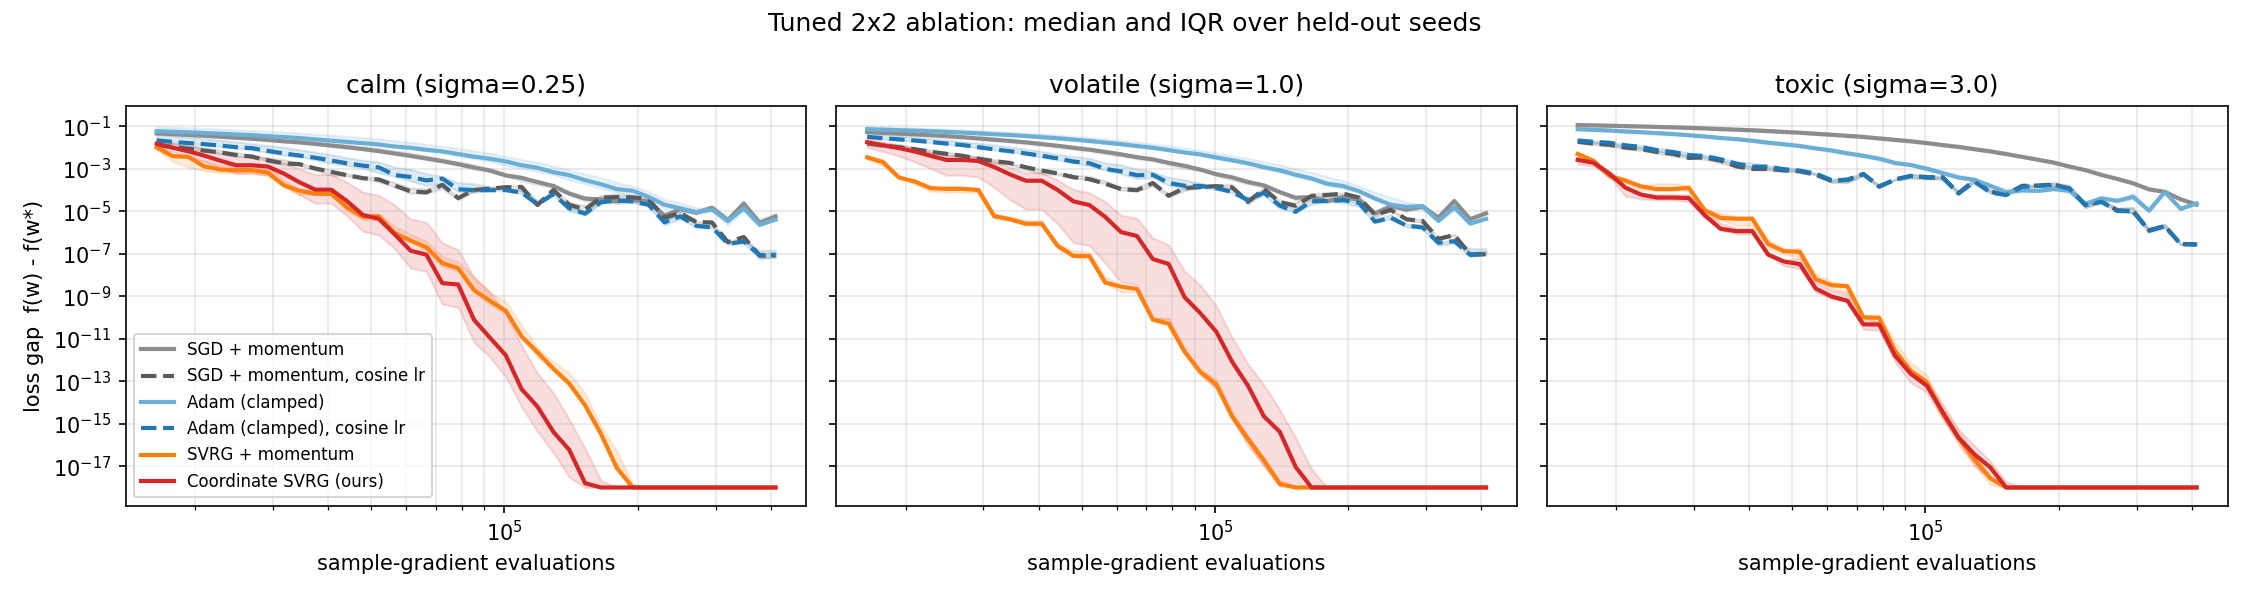
\includegraphics[width=\linewidth]{ablation_curves.png}
\caption{Least squares, three noise regimes: loss gap against sample-gradient evaluations (median and IQR over held-out seeds). Curves are clamped at $10^{-18}$ for plotting.}
\end{figure}

\subsection{Adaptive scaling helps only when features are badly scaled}
With column scales spread over three decades (Table~\ref{tab:hetero}), Coordinate SVRG at a constant rate has a median paired difference of \ExpSixAdaptiveVsMomentum{} decades against SVRG with plain momentum (negative favours Coordinate SVRG; 95\% CI \ExpSixAdaptiveCI, better on \ExpSixAdaptiveWins{} seeds), yet plateaus at a median gap of $\ExpSixConstGap$, as anticipated in Section~\ref{sec:theory}. Adding cosine decay removes the plateau (median $\ExpSixCosineGap$) and beats the best tuned baseline, Adam with cosine decay ($\ExpSixAdamCosineGap$): paired difference \ExpSixCosineVsAdamCosine{} decades (CI \ExpSixCosineCI, better on \ExpSixCosineWins{} seeds). On well-scaled data the adaptive component does not help and, at constant rate on the larger problem, hurts. Proposition~\ref{prop:precond} predicts this pattern through $\kappa_D$.

\begin{figure}[h]
\centering
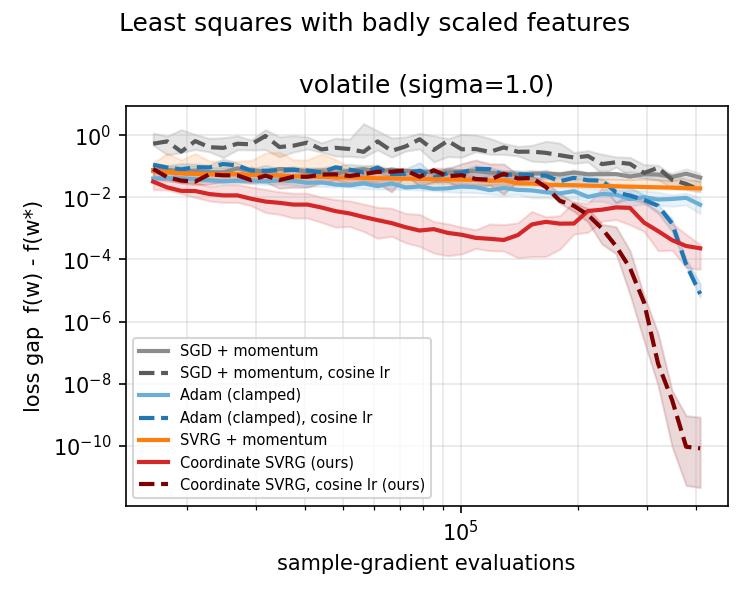
\includegraphics[width=0.6\linewidth]{hetero_curves.png}
\caption{Badly scaled features. Among these methods, only variance reduction with adaptive scaling and a decaying rate reaches the target; Section~\ref{sec:jacobi} adds a simpler method that does better.}
\end{figure}

\subsection{The variance law along a real trajectory}
Along one run (Figure~\ref{fig:var}), mini-batch SGD variance stays between \ExpTwoSgdMin{} and \ExpTwoSgdMax{}, while the variance of $\ghat$ falls from $\ExpTwoVrStart$ to $\ExpTwoVrEnd$. In all \ExpTwoProbes{} probes, each at worst-case snapshot staleness, measured variance was within the Lemma~\ref{lem:var} bound (\ExpTwoWithinLemma\%) and the Proposition~\ref{prop:stale} bound (\ExpTwoWithinProp\%).

\begin{figure}[h]
\centering
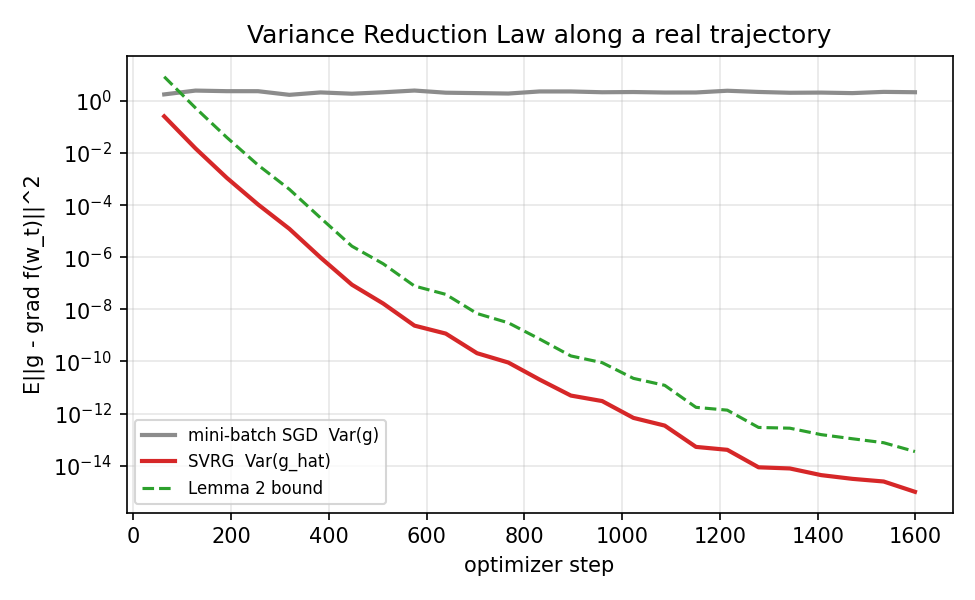
\includegraphics[width=0.55\linewidth]{variance_decay.png}
\caption{Gradient variance along the trajectory, with the Lemma~\ref{lem:var} bound.}\label{fig:var}
\end{figure}

\subsection{Non-convex fit: sharper stationarity, worse generalisation}
For a one-hidden-layer tanh network the squared full-gradient norm of Coordinate SVRG with cosine decay is lower than the best baseline's by \ExpSevenDecades{} decades in $\log_{10}$ (negative means lower; \ExpSevenWins{} seeds). On a held-out random split, however, with learning rates tuned on training loss, its test loss is \ExpEightSvrgTest{} against \ExpEightBaselineTest{} for \ExpEightBaselineName{} (paired difference \ExpEightGap, 95\% CI \ExpEightCI; the noise floor is $0.125$), while its training loss is lower (\ExpEightSvrgTrain{} against \ExpEightBaselineTrain). It fits the training noise harder. Tuning on validation loss could change the ranking. For held-out logistic regression all methods are indistinguishable (test log-loss \ExpEightLogisticLow{} to \ExpEightLogisticHigh, about \ExpEightAccuracy\% accuracy).

\subsection{Snapshot interval and wall-clock}
Evaluations to the target are U-shaped in the snapshot interval $K$: best at $K=\ExpNineBestK$ (\ExpNineBestEvals{} evaluations), within a factor \ExpNineMidFactor{} for $16\le K\le256$, \ExpNineSmallFactor$\times$ worse at $K=\ExpNineKmin$ and \ExpNineLargeFactor$\times$ worse at $K=\ExpNineKmax$ (Figure~\ref{fig:si}). On a larger problem ($n=\ExpFiveN$, $d=\ExpFiveD$) SVRG with momentum reaches the target in \ExpFiveSvrgSeconds\,s on one NumPy core, whereas the normal equations take \ExpFiveNormalSeconds\,s and \texttt{lstsq} \ExpFiveLstsqSeconds\,s: a direct solve still matches SVRG at this size, and the iterative timing excludes the cost of tuning the learning rate.

\begin{figure}[h]
\centering
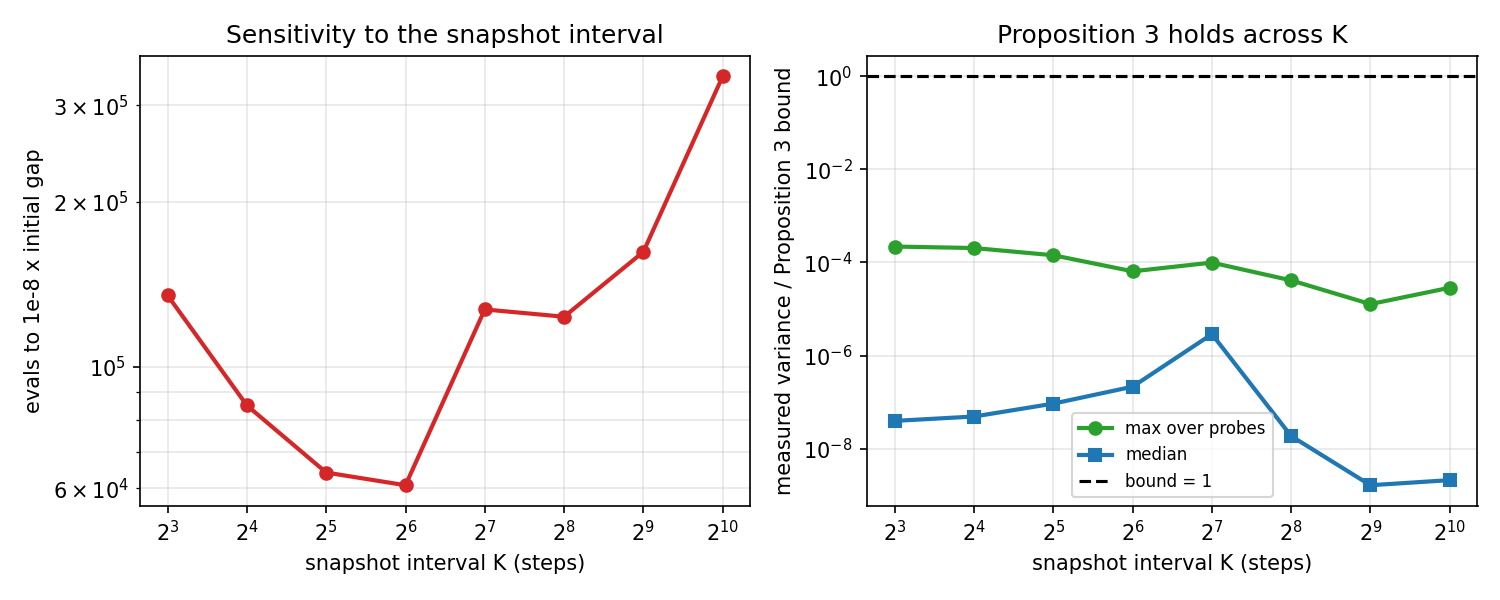
\includegraphics[width=0.9\linewidth]{snapshot_interval.png}
\caption{Sensitivity to the snapshot interval, and the Proposition~\ref{prop:stale} ratio across intervals.}\label{fig:si}
\end{figure}

\subsection{A method read off the theory}\label{sec:jacobi}
Proposition~\ref{prop:precond} suggests using the frozen Jacobi preconditioner $D=\mathrm{diag}(X^\top X/n)$ and taking every other hyper-parameter from the Johnson--Zhang recipe: $\eta=0.1/L_D$, $m=\lceil 50L_D/\gamma_D\rceil$ single-sample inner steps ($m=\ExpElevenInner$ here), random-iterate snapshots, for a guaranteed per-epoch contraction factor $\alpha=\ExpElevenAlpha$ and \emph{no tuning}. On the datasets and seeds of Tables~\ref{tab:ls} and~\ref{tab:hetero} (Table~\ref{tab:jacobi}), this reaches $\ExpElevenBadTheoryGap$ on the badly scaled problem, at float64 round-off, beating Coordinate SVRG with cosine decay ($\ExpSixCosineGap$) on \ExpElevenBadWins{} seeds and needing \ExpElevenEvalsTheory{} sample-gradient evaluations to reach the target against \ExpElevenEvalsCoord{} for that method (\ExpElevenSpeedup$\times$ fewer). The measured mean epoch-to-epoch contraction is \ExpElevenContractionBad{} (badly scaled) and \ExpElevenContractionGood{} (well-scaled), consistent with the guaranteed $\ExpElevenAlpha$ in expectation but loose by a factor of about five. On well-scaled data it matches the other round-off-level methods.
Does the finding carry beyond least squares? On $\ell_2$-regularised logistic regression with the same three-decade feature scaling (\ExpTwelveSeeds{} held-out seeds, Hessian-diagonal upper bound $D=\tfrac14\,\mathrm{mean}(x^2)+\ell_2$, learning rate tuned like every other method), tuned Jacobi SVRG again reaches round-off (median $\ExpTwelveJacobiGap$) and beats Coordinate SVRG with cosine decay ($\ExpTwelveCoordGap$) on \ExpTwelveWins{} seeds, needing \ExpTwelveEvalsJacobi{} evaluations to the target against \ExpTwelveEvalsCoord{} (\ExpTwelveSpeedup$\times$ fewer); tuned Adam with cosine decay stops at $\ExpTwelveAdamCosineGap$. Two nuances: this run is tuned, not theory-prescribed, because the global strong-convexity modulus of the logistic loss is only the $\ell_2$ weight and the worst-case recipe is far too conservative to be informative; and on this problem constant-rate Coordinate SVRG does \emph{not} plateau and has a paired difference of \ExpTwelveAdaptiveVsMomentum{} decades against SVRG with plain momentum, so the plateau seen in the least-squares case is problem-dependent.
The comparison favours Jacobi-SVRG in one respect that should be stated: it uses the Hessian diagonal of a linear model, one extra pass over the data not charged above, whereas Coordinate SVRG uses gradients only and applies to models where the Hessian diagonal is unavailable. The finding is that where the Hessian diagonal \emph{is} available, the simpler theory-derived method dominates the more elaborate one.

\begin{figure}[ht]
\centering
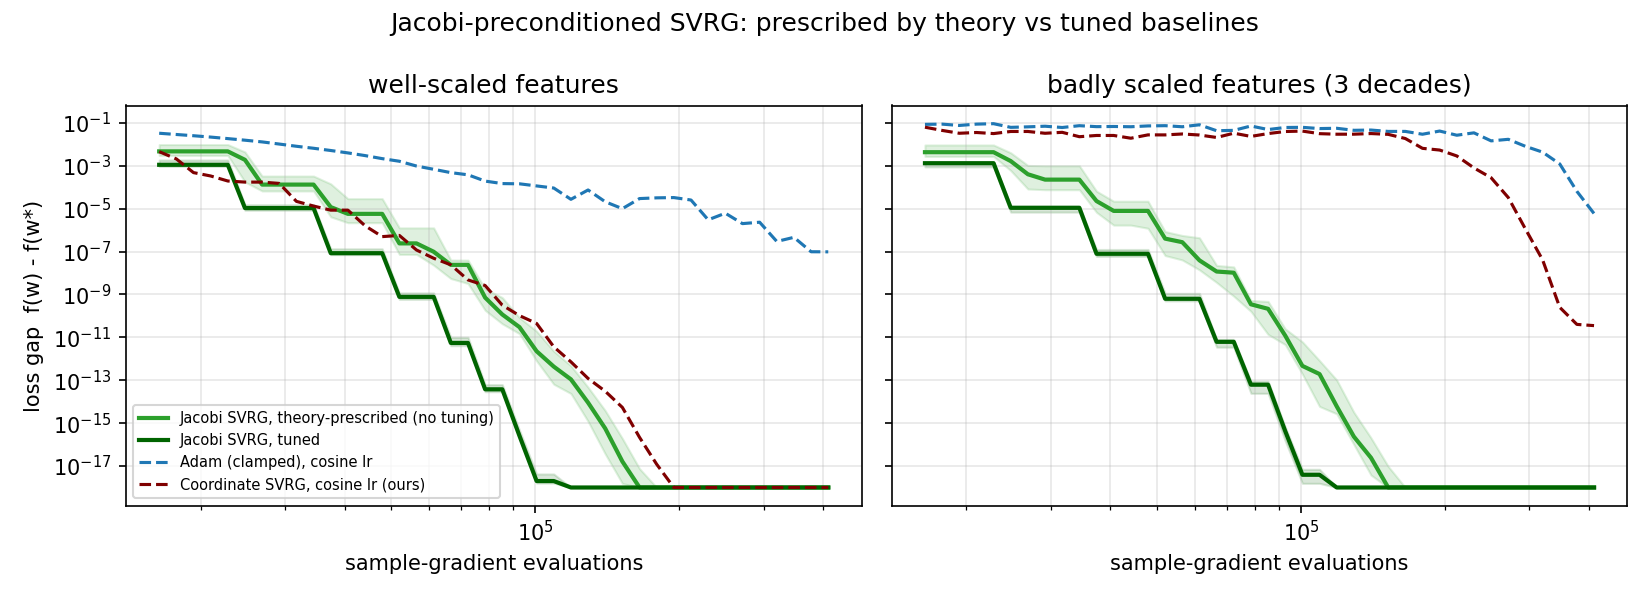
\includegraphics[width=0.95\linewidth]{jacobi_curves.png}
\caption{Jacobi-preconditioned SVRG (theory-prescribed and tuned) against the best tuned baselines.}
\end{figure}

\subsection{Real data with raw features}\label{sec:real}
To check that the findings are not artefacts of the simulator, I ran the same protocol on three bundled real datasets with raw, unstandardised features plus an intercept (Table~\ref{tab:real}): breast-cancer diagnosis and wine (logistic regression) and diabetes progression (least squares). Their feature scales span \ExpThirteenBCDecades{} decades (breast cancer) down to 1.8 decades, and Jacobi scaling reduces the condition number of the Hessian at the optimum by two to three orders of magnitude (breast cancer: $\ExpThirteenBCCondRaw\to\ExpThirteenBCCondJacobi$).
Two results carry over and one does not. Preconditioned methods (Jacobi SVRG, Coordinate SVRG, Adam) beat the unpreconditioned ones (SGD, SVRG with momentum) by large margins on all three. Jacobi SVRG has the lowest median gap on wine and diabetes and is tied with Coordinate SVRG with cosine decay on breast cancer (medians differing by 0.2\%); its margin over the best tuned baseline is small, between \ExpThirteenMinDiff{} and \ExpThirteenMaxDiff{} decades. What does \emph{not} carry over is the round-off result: no method reached the $10^{-8}$ target within 1000 epochs on any dataset, because $\kappa$ remains large even after Jacobi scaling and the datasets are tiny. Three datasets cannot support a general claim, the seeds vary only the batch order (so the intervals say nothing about variation across datasets), and one baseline learning rate (diabetes, Adam with cosine decay) sat on the edge of its grid.

\subsection{Walk-forward signal tracking: no benefit}
In a rolling re-estimation of a drifting alpha under a compute budget, every method's out-of-sample correlation with the clean signal differs from closed-form OLS by at most \ExpThreeMaxICDiff, against a spread across datasets of about \ExpThreeIQR; paired intervals often exclude zero but the effects are negligible, and SVRG never beats Adam. The problem is too small for the choice of optimizer to matter.

\section{Ablating the invariants}\label{sec:invariants}
\paragraph{Sample alignment (invariant 2).} Taking the snapshot gradient on an \emph{independent} batch instead of the same one destroys the control variate (Figure~\ref{fig:align}). At snapshot distance $0.01$ the estimator's mean squared error is $\ExpFourteenAligned$ with aligned batches, $\ExpFourteenMisaligned$ with misaligned batches, and $\ExpFourteenSgd$ for plain mini-batch SGD: misaligned SVRG is $\ExpFourteenRatio\times$ \emph{worse than not using variance reduction}, and its error does not shrink with distance.
\begin{figure}[h]
\centering
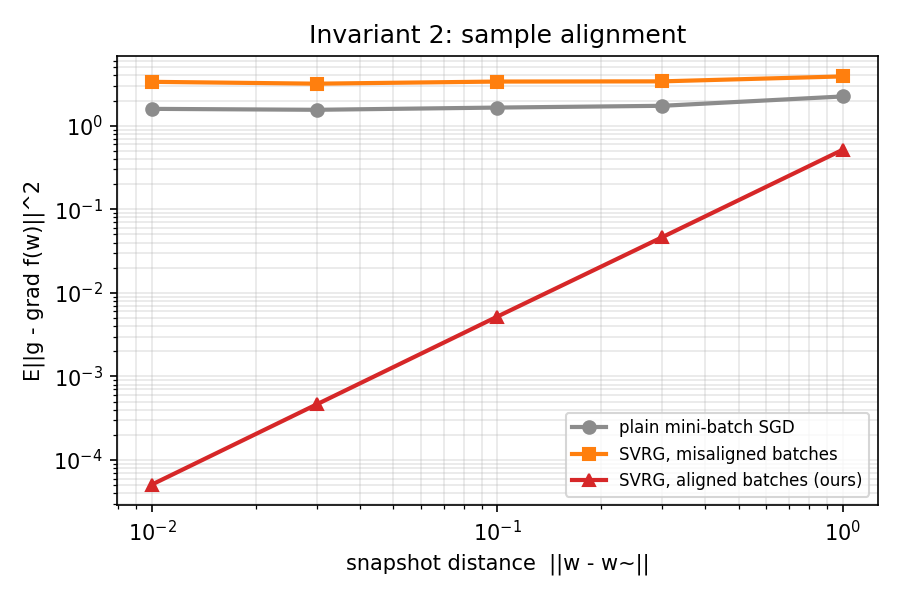
\includegraphics[width=0.55\linewidth]{alignment_violation.png}
\caption{Gradient-estimator error against snapshot distance, with aligned and misaligned batches.}\label{fig:align}
\end{figure}
\paragraph{Coordinate safeguards (invariant 4).} In \ExpFourteenTrials{} adversarial float32 trials (10 steps, momentum and decay up to $0.9999$, gradients drawn from zeros, denormals and values up to $3\times10^{38}$, and in a second tier also infinities and NaN), textbook Adam with an additive $\varepsilon$ produced non-finite weights in \ExpFourteenNaiveFinite\% of trials with extreme but finite inputs and \ExpFourteenNaiveInf\% with infinities or NaN; a clamp-only variant failed identically (\ExpFourteenClampFinite\%); the full guard set failed in \ExpFourteenFullFinite\%. The operative guard is therefore the sanitising and bounding of the gradient; the denominator floor alone adds nothing in this test. (An earlier version of this work claimed that clamping rather than offsetting the denominator mattered; this experiment shows it does not.) The inputs are deliberately hostile and describe a robustness guarantee, not typical training.

\section{Limitations and threats to validity}
\begin{itemize}[leftmargin=*,itemsep=2pt]
\item \textbf{Mostly synthetic data.} The simulator generates what the models assume, and the only real data are three small non-financial datasets on which the round-off results do not reproduce. Nothing here is evidence of real-market performance.
\item \textbf{Convex bias.} Most experiments are convex, the best case for SVRG; variance reduction is known to help far less in deep learning \cite{defazio2019}. One small non-convex network is not evidence about deep models.
\item \textbf{Scale.} The largest problem has $n=\ExpFiveN$, $d=\ExpFiveD$, where a direct solve is as fast as any iterative method.
\item \textbf{Engines versus experiments.} The PyTorch and JAX engines passed the full test suite (58 tests at the time, the later real-market-study tests not yet run there), including step-for-step agreement with the oracle, on a Colab T4 runtime; on the GPU the PyTorch engine stayed within $1.8\times10^{-7}$ of the oracle over 100 steps, and a 640-step benchmark's final loss gaps matched the oracle to four significant digits. The reported experiment numbers nevertheless come from the NumPy oracle, and no timing or speed study was done.
\item \textbf{No convergence proof for the adaptive engine}; the cosine-decay results are empirical.
\item \textbf{Statistics.} Seed counts range from 3 to 20; intervals are bootstrap intervals over seeds; no multiple-comparison correction; learning rates are tuned on training loss in the non-convex and logistic held-out checks.
\item \textbf{Tuning cost} is excluded from the iterative wall-clock times.
\item \textbf{Jacobi-SVRG scope.} It needs the Hessian diagonal, available for linear and generalised-linear models but not in general. It was tested on least squares (theory-prescribed and tuned) and logistic regression (tuned only), its single-sample theory variant is slow per evaluation in wall-clock terms, and the evaluation counts above do not charge the one extra pass that computes $D$.
\end{itemize}

\section{Reproducibility}
The repository fixes every random stream from one seed. \texttt{make test} runs the invariant, oracle, differential and fuzz tests; \texttt{make experiments} regenerates all results and figures; \texttt{make report} rebuilds this document, whose numbers are macros generated from \texttt{results/experiments.json}. A continuous-integration workflow runs the tests on CPU PyTorch and JAX. \texttt{experiments/real\_market\_study.py} provides a purged walk-forward study on real daily returns with a placebo run; no results from it are reported here.

\begin{thebibliography}{9}
\bibitem{johnson2013} R.~Johnson, T.~Zhang. Accelerating stochastic gradient descent using predictive variance reduction. \emph{NeurIPS}, 2013.
\bibitem{kingma2015} D.~Kingma, J.~Ba. Adam: a method for stochastic optimization. \emph{ICLR}, 2015.
\bibitem{reddi2018} S.~Reddi, S.~Kale, S.~Kumar. On the convergence of Adam and beyond. \emph{ICLR}, 2018.
\bibitem{defazio2019} A.~Defazio, L.~Bottou. On the ineffectiveness of variance reduced optimization for deep learning. \emph{NeurIPS}, 2019.
\bibitem{vandersluis1969} A.~van der Sluis. Condition numbers and equilibration of matrices. \emph{Numerische Mathematik} 14, 1969.
\end{thebibliography}

\end{document}
